%%%% Proceedings format for most of ACM conferences (with the exceptions listed below) and all ICPS volumes.
\documentclass[sigconf]{acmart}
\usepackage{graphicx, wrapfig}
\graphicspath{{imgs/}}
\usepackage{lipsum}
\usepackage{stfloats}
\usepackage{enumerate}
\usepackage[most]{tcolorbox}
\usepackage[english,ngerman,brazilian]{babel}


\newtcolorbox[blend into=figures]{card}[2][]{enhanced,
  float=tbp,title={#2},
  colframe=gray!75!black,olback=yellow!5!white,#1
}


\settopmatter{printacmref=false}
\setcopyright{none}
\renewcommand\footnotetextcopyrightpermission[1]{}
\pagestyle{plain}
\captionsetup{justification   = raggedright,
              singlelinecheck = false}
\newcommand{\source}[2]{\raggedleft{}\vspace*{-7mm}\caption*{ \textmd{\scriptsize{Dados: {#1}.\hfill Ferramenta:{#2}}}}}
\def\BibTeX{{\rm B\kern-.05em{\sc i\kern-.025em b}\kern-.08emT\kern-.1667em\lower.7ex\hbox{E}\kern-.125emX}}

% end of the preamble, start of the body of the document source.
\begin{document}

%
% The "title" command has an optional parameter, allowing the author to define a "short title" to be used in page headers.
\title[Fronteiras da Transferência de Aprendizado: uma revisão sistemática com enfoque meta-analítico]{Fronteiras da Transferência de Aprendizado: \\
uma revisão sistemática com enfoque meta-analítico}
%

\author{Fred Guth}
\email{fredguth@fredguth.com}
\affiliation{%
  \institution{Departamento de Ciência de Computação, Universidade de Brasília}
  \postcode{70.910-900}
  \city{Brasília}
  \state{DF}
  \country{Brazil}
}

\renewcommand{\shortauthors}{Guth, F.}

\begin{abstract}
  Humanos e animais conseguem aprender com poucas amostras \cite{goodfellow} e apresentam extraordinária capacidade de generalização que os algoritmos de aprendizagem de máquina ainda estão longe de alcançar. Os modelos mais bem sucedidos da atualidade exigem uma enormidade de dados bem rotulados que são caros e difíceis de obter, tornando-se hoje um dos maiores empecilhos para aplicações práticas. Tais fatos apontam para o grande potencial da área de Transferência de Aprendizado, que tem por objetivo aproveitar o conhecimento obtido em uma atividade para aprender mais eficientemente outras, que guardem alguma relação com a primeira. O presente estudo visa apresentar uma revisão sistemática da literatura e identificar, com embasamento quantitativo, as principais contribuições para a área. Além disso, usamos medidas de acoplamento bibliográfico para identificar trabalhos na fronteira do conhecimento e fizemos uma análise textual, em resumos e palavras-chave, comparando estes com os "clássicos" da área de forma a mapear para que direção a pesquisa avança.  
\end{abstract}


\begin{CCSXML}
<ccs2012>
 <concept>
 <concept_id>10010147.10010257.10010258.10010262.10010277</concept_id>
 <concept_desc>Computing methodologies~Transfer learning</concept_desc>
 <concept_significance>500</concept_significance>
 </concept>
</ccs2012>
\end{CCSXML}
\ccsdesc[500]{Computing methodologies~Transfer learning}

\keywords{transferência de aprendizado, revisão sistemática, enfoque meta-analítico}


\maketitle


\section{Introdução} 
  Recentes avanços em Aprendizagem de Máquina tornam possíveis aplicações que são capazes de reconhecer pessoas, lugares e objetos com acurácia super-humana\cite{fei}, diagnosticar câncer de pele tão bem quanto dermatologistas\cite{skin_cancer},  ver através de paredes usando sinais de rádio\cite{wifi}, entre tantas outras. Apesar de tanto sucesso, os modelos mais bem sucedidos da atualidade exigem uma enormidade de dados bem rotulados que são caros e difíceis de obter, pois, em geral, o jeito padrão de se treinar modelos é sempre começar \emph{tabula rasa}, ou seja, com uma inicialização aleatória dos parâmetros. 
  
  Aprender assim, a partir do nada, é contrário à forma como os humanos o fazem. Em nosso dia a dia, transferimos conhecimento a todo momento. Saber tocar piano, facilita aprender tocar órgão. Reconhecer maçãs talvez ajude a reconhecer peras. Pessoas conseguem inteligentemente aplicar conhecimento prévio para resolver novos problemas com maior eficácia e eficiência\cite{PanYang}. Algoritmos de aprendizagem de máquina ainda estão longe de alcançar essa extraordinária capacidade de generalização\cite{goodfellow}. Estudos recentes~\cite{DBLP:journals/corr/JiaL17}, mostram que os algoritmos atuais não generalizam bem além de dados vistos durante o treinamento.
  \begin{figure}[h]
    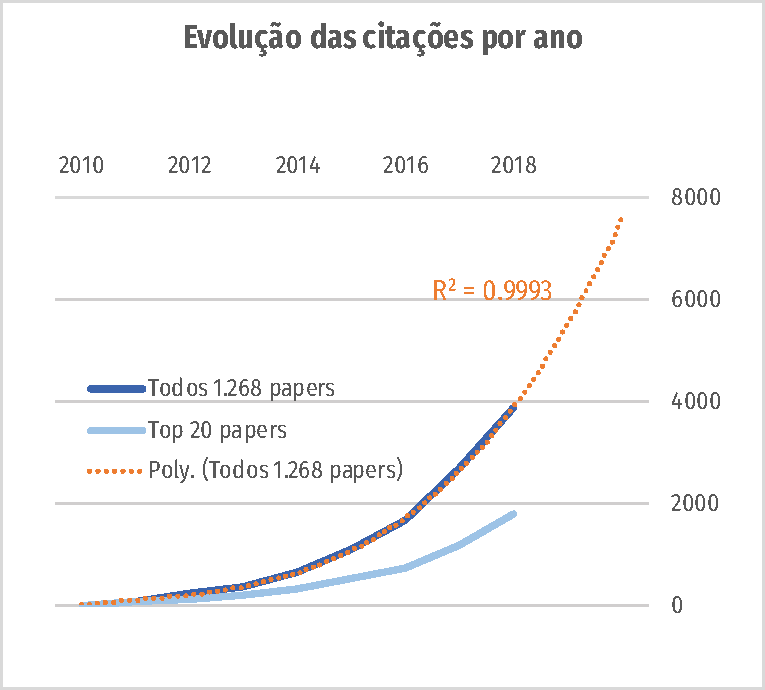
\includegraphics[width=\columnwidth]{citacoes_por_ano2.pdf}
    \source{Web of Science (março/2019)}{Excel}
    \caption{Evolução dos número de citações de artigos em Tranferência de Aprendizagem nos últimos 10 anos.}
    \label{fig:citacoes_por_ano}
  \end{figure}
  
  Tais fatos apontam  o grande potencial ainda inalcançado da área de Transferência de Aprendizado (TL\footnote{Do inglês \emph{Transfer Learning}}), que tem por objetivo aproveitar o conhecimento obtido em uma atividade para aprender mais eficientemente outras, que guardem alguma relação com a primeira.
  
  Na prática, entretanto, TL ainda é tratada de uma forma \textit{ad hoc}, sendo os métodos de transferências meras extensões dos algoritmos de aprendizado utilizados \cite{torrey}. Essa dicotomia entre a importância do problema e a inexistência de práticas e teorias consolidadas, tornam TL um campo promissor e interessante para pesquisa. 
  
  \begin{quote} "Transferência de Aprendizado será o próximo motor do sucesso comercial com Aprendizado de Máquinas." \hfill ---Andrew Ng, Tutorial NIPS 2016 \cite{ANg}
  \end{quote}

  Portanto, não é de se estranhar o crescente interesse pelo assunto (vide \S\ref{sec:panorama} e figura \ref{fig:citacoes_por_ano}).  

  \subsection{Objetivo}
   Esta pesquisa quer responder duas perguntas:
    \begin{enumerate}
      \item{Quais são as fronteiras do conhecimento em Transferência de Aprendizagem?}
      \item {É possível embasar essa avaliação em dados bibliométricos?}
    \end{enumerate}
    Para responder estas perguntas é preciso, antes, analisar a literatura do tema, revelar as principais contribuições e como se relacionam.
  
  \subsection{Contribuições}

    \begin{enumerate}[C1.]
      \item Apresentamos uma revisão sistemática atualizada da literatura em Transferência de Aprendizagem, usando a abordagem TEMAC (\S \ref{TEMAC}). Esse método nos permite focar nas contribuições de alto impacto. 
      \item Estendemos o TEMAC com uma análise textual de resumos (\S \ref{analiseTextual}), utilizando o ScatterText, até onde sabemos, é uma aplicação original desta ferramenta de visualização.
      \item Apontamos com embasamento quantitativo as direções das frentes de pesquisa da área e apontamos lacunas e problemas em aberto.
    \end{enumerate}
  
  \subsection{Visão Geral e Organização do Artigo}
  \lipsum[3]
  \subsection{Trabalhos Relacionados}
  \lipsum[2]
\section{Método: Revisão com Enfoque Meta-Analítico Consolidado}\label{TEMAC}
Na presente pequisa utilizamos o método de revisão sistemática da Teoria do Enfoque Meta-Analítico (TEMAC) ~\cite{Mariano}, que visa oferecer um embasamento quantitativo para a escolha da literatura. Apesar do nome, TEMAC não deve ser confundida com Meta-Análise, pois o foco desta é gerar conhecimento por meio de dados empíricos secundários, enquanto o daquela é oferecer uma sistematização da escolha bibliográfica.

A abordagem TEMAC é dividida em 3 etapas: 
\begin{enumerate}[a)]
  \item preparação da pesquisa;
  \item apresentação e inter-relação dos dados;
  \item detalhamento, modelo integrador e validação por evidências.
\end{enumerate}

\subsection{Preparação da Pesquisa}
Foi realizada uma busca na base de dados \emph{Clarivate Analyticis Web of Science (WoS)}, conforme especificado na figura \ref{card:wos}, no dia 31 de março de 2019, que resultou em 1.289 artigos encontrados. Nota-se que o tema é de crescente interesse (figura \ref{fig:citacoes_por_ano}) e projeta-se que em 2 anos o número de citações irá praticamente dobrar (crescimento cubico com R-quadrado 0,9993).
\begin{figure}[htp]

\begin{tcolorbox}[colback=yellow!5!white,colframe=gray!75!black,title={Results: 1,289 (from Web of Science Core Collection)}]
  \begin{verbatim}
  You searched for: 
  TOPIC: ("transfer learning")
  Refined by: 
  WEB OF SCIENCE CATEGORIES: 
    ( COMPUTER SCIENCE ARTIFICIAL INTELLIGENCE )
  AND LANGUAGES: ( ENGLISH ) 
  AND RESEARCH AREAS: ( COMPUTER SCIENCE )
  Timespan: 2009-2019. 
  Indexes: SCI-EXPANDED, CPCI-S, ESCI.
  \end{verbatim}

\end{tcolorbox}
\caption{Parâmetros de busca na base \emph{Web of Science}.}
\label{card:wos}
\end{figure}

Também fizemos uma busca mais restrita (figura \ref{card:sota}) aos trabalhos mais recentes para a análise da Fronteira de pesquisa (\S \ref{fronteira}).
\begin{figure}[htp]
  \begin{tcolorbox}[colback=yellow!5!white,colframe=gray!75!black,title={Results: 161 (from Web of Science Core Collection)}]
  \begin{verbatim}
  You searched for: 
  TOPIC: ("transfer learning")
  Refined by: 
  WEB OF SCIENCE CATEGORIES: 
    ( COMPUTER SCIENCE ARTIFICIAL INTELLIGENCE )
  AND LANGUAGES: ( ENGLISH ) 
  AND RESEARCH AREAS: ( COMPUTER SCIENCE )
  AND PUBLICATION YEARS: ( 2019 OR 2018 )
  AND DOCUMENT TYPES: ( PROCEEDINGS PAPER )
  Timespan: 2009-2019. 
  Indexes: SCI-EXPANDED, CPCI-S, ESCI.
  \end{verbatim}

  
  \end{tcolorbox}
  \caption{Parâmetros de busca para análise de Fronteira.}
  \label{card:sota}
\end{figure}

\subsection{Apresentação e Inter-relação dos Dados}
O software livre \emph{VosViewer 1.6.10}~\cite{VOSviewer} foi utilizado para as análises bibliográficas. Ele permite analisar co-citação e acoplamento bibliográfico de documentos e autores. Para análise textual de resumos utilizamos a ferramenta \emph{ScatterText}~\cite{kessler2017scattertext}.

\begin{enumerate}[a)]
  \item{\textbf{Análise de Co-citações}: Co-citação é definida como a frequência em que dois documentos são citados em uma mesma lista de referências. Assume-se que são "peças"~que compõem uma mesma "estrutura de conhecimento".  A análise de co-citações, portanto, é útil para mapear a herança intelectual de um determinado campo de estudos sob a ótica das publicações de alto-impacto, mas tende a negligenciar a dinâmica na fronteira de pesquisa\cite{Vogel2012}, justamente porque os trabalhos na fronteira não tiveram tempo para serem citados e pontuar nas métricas de impacto. }
    
    
  \item{\textbf{Análise de Acoplamento Bibliográfico}: Acoplamento bibliográfico ocorre quando dois documentos tem pelo menos um documento em comum, ou seja, documentos acoplam se suas bibliografias se sobrepõem. Como existe uma ordem cronológica entre o documento que cita e o que é citado, o acoplamento bibliográfico permite traçar gerações de pesquisas e com isso identificar as que estão na fronteira do conhecimento.  É importante ressaltar que, neste contexto, estar na fronteira não é necessariamente ser promissor. Essa é uma limitação da abordagem quantitativa, por isso é preciso complementá-la com uma análise qualitativa para propor, ainda que com certo grau de subjetividade, os trabalhos promissores a se tornar os "clássicos de amanhã".
  Pelo TEMAC, a análise de acoplamento bibliográfico deve ser feita para o período um período não superior aos últimos 3 anos. Em nossa análise, usamos uma busca mais restrita (figura \ref{card:sota}) com período entre 2018 e março de 2019.
  }
  \item{\textbf{Análise tf-idf}: neste trabalho, usamos o conceito de \textbf{tf-idf} para definir as palavras que melhor identificam determinados documentos. Por exemplo, quais palavras melhor explicam trabalhos de fronteira vis à vis o todos os documentos resultantes da busca na base \emph{Web of Science} (vide figura \ref{fig:scatterText}). A métrica \textbf{tf-idf} pode ser definida como:
  \begin{equation}
    \mathrm{tfidf}(t,d,D) = \mathrm{tf}(t,d) \cdot \mathrm{idf}(t, D)
  \end{equation}
  onde $\mathrm{tf}(t,d)$ é a frequência em que um termo $t$ aparece em um documento $d$ e $\mathrm{idf}(t, D)$ é o inverso da frequência do termo $t$ no conjunto de documentos $D$ (o \emph{corpus}). 
  \begin{equation}
    \mathrm{tf}(t,d) = 0.5 + 0.5 \cdot  \frac{f_{t, d}}{\max\{f_{t', d}:t' \in d\}}
  \end{equation}
  \begin{equation}
    \mathrm{idf}(t, D) =  \log \frac{N}{|\{d \in D: t \in d\}|}
  \end{equation}
  onde:
  \begin{description}
    \item $N$: número de documentos do corpus $N = {|D|}$
   \item$ |\{d \in D: t \in d\}| $ : número de documentos onde o termo  $ t $ aparece (i.e., $ \mathrm{tf}(t,d) \neq 0$). Para evitar uma divisão por zero caso o termo não esteja no corpus, é como fazer um ajuste no denominador para: $1 + |\{d \in D: t \in d\}|$.
   
   
  \end{description}
  }\label{analiseTextual}
\end{enumerate}


\begin{figure*}[b]
  \centering
  \fbox{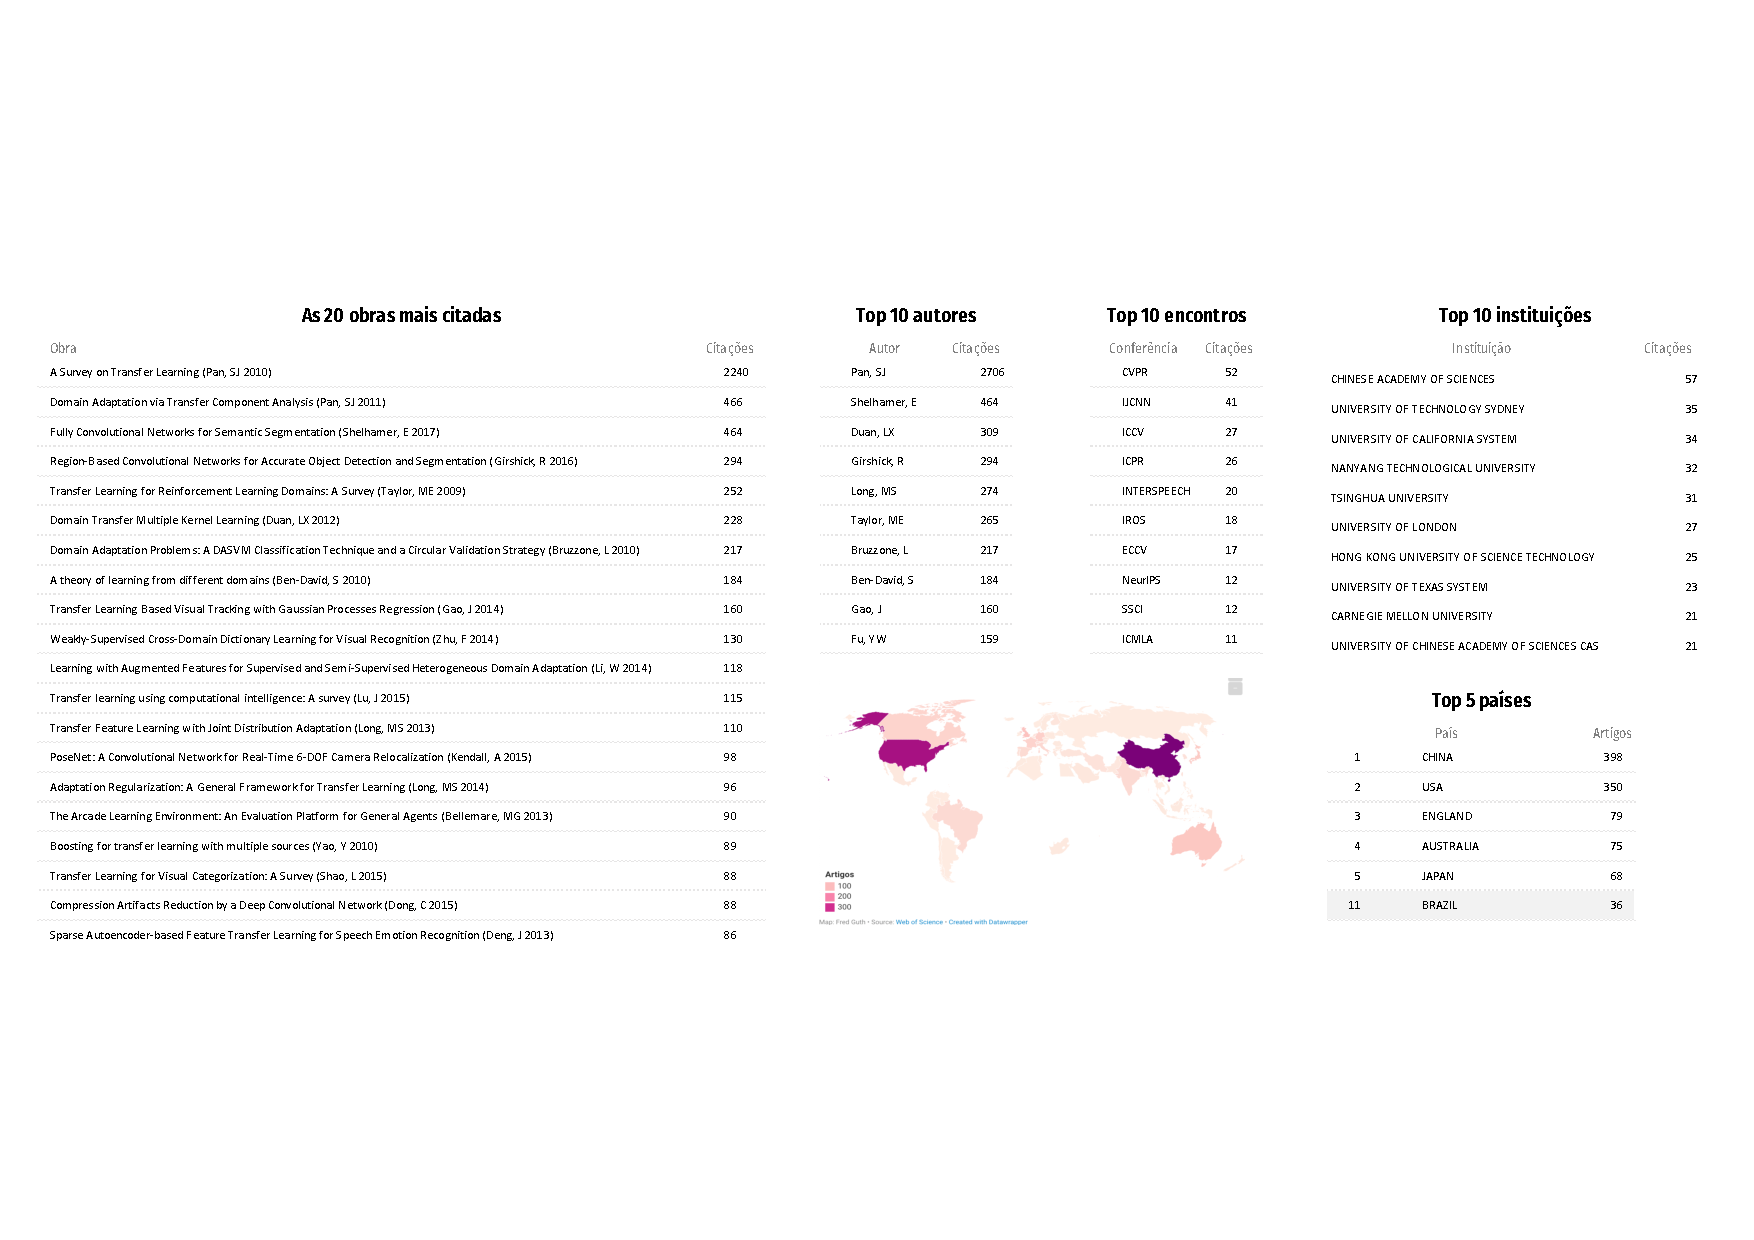
\includegraphics[width=\textwidth]{listas.pdf}}
  \source{Web of Science (março/2019)}{Excel}
  \caption{Panorama da produção científica sobre Transferência de Aprendizagem.} \label{fig:toptop}
\end{figure*}
\section{Revisão da Literatura}
  \subsection{Transferência de Aprendizagem}
  \lipsum[3]
  \subsection{Um breve histórico}
  Pesquisa em transferência de aprendizagem tem atraído mais e mais atenção desde 1995, quando foi tema de  um workshop na NIPS-95 que discutiu a necessidade de métodos de aprendizado de máquina que retém e reusam conhecimento previamente obtido~\cite{PanYang}. 
  
  ImageNet’s impact on the course of machine learning research can hardly be overstated. The dataset was originally published in 2009 and quickly evolved into the ImageNet Large Scale Visual Recognition Challenge (ILSVRC). In 2012, the deep neural network submitted by Alex Krizhevsky, Ilya Sutskever, and Geoffrey Hinton performed 41% better than the next best competitor, demonstrating that deep learning was a viable strategy for machine learning and arguably triggering the explosion of deep learning in ML research.

The success of ImageNet highlighted that in the era of deep learning, data was at least as important as algorithms. Not only did the ImageNet dataset enable that very important 2012 demonstration of the power of deep learning, but it also allowed a breakthrough of similar importance in transfer learning: researchers soon realized that the weights learned in state of the art models for ImageNet could be used to initialize models for completely other datasets and improve performance significantly. This "fine-tuning" approach allowed achieving good performance with as little as one positive example per category (Donahue et al., 2014)

  \subsection{O panorama da produção científica na área}\label{sec:panorama}
 
  \lipsum[1]
  
  

 
  \subsection{Os Clássicos}
  \begin{figure}[h]
    \fbox{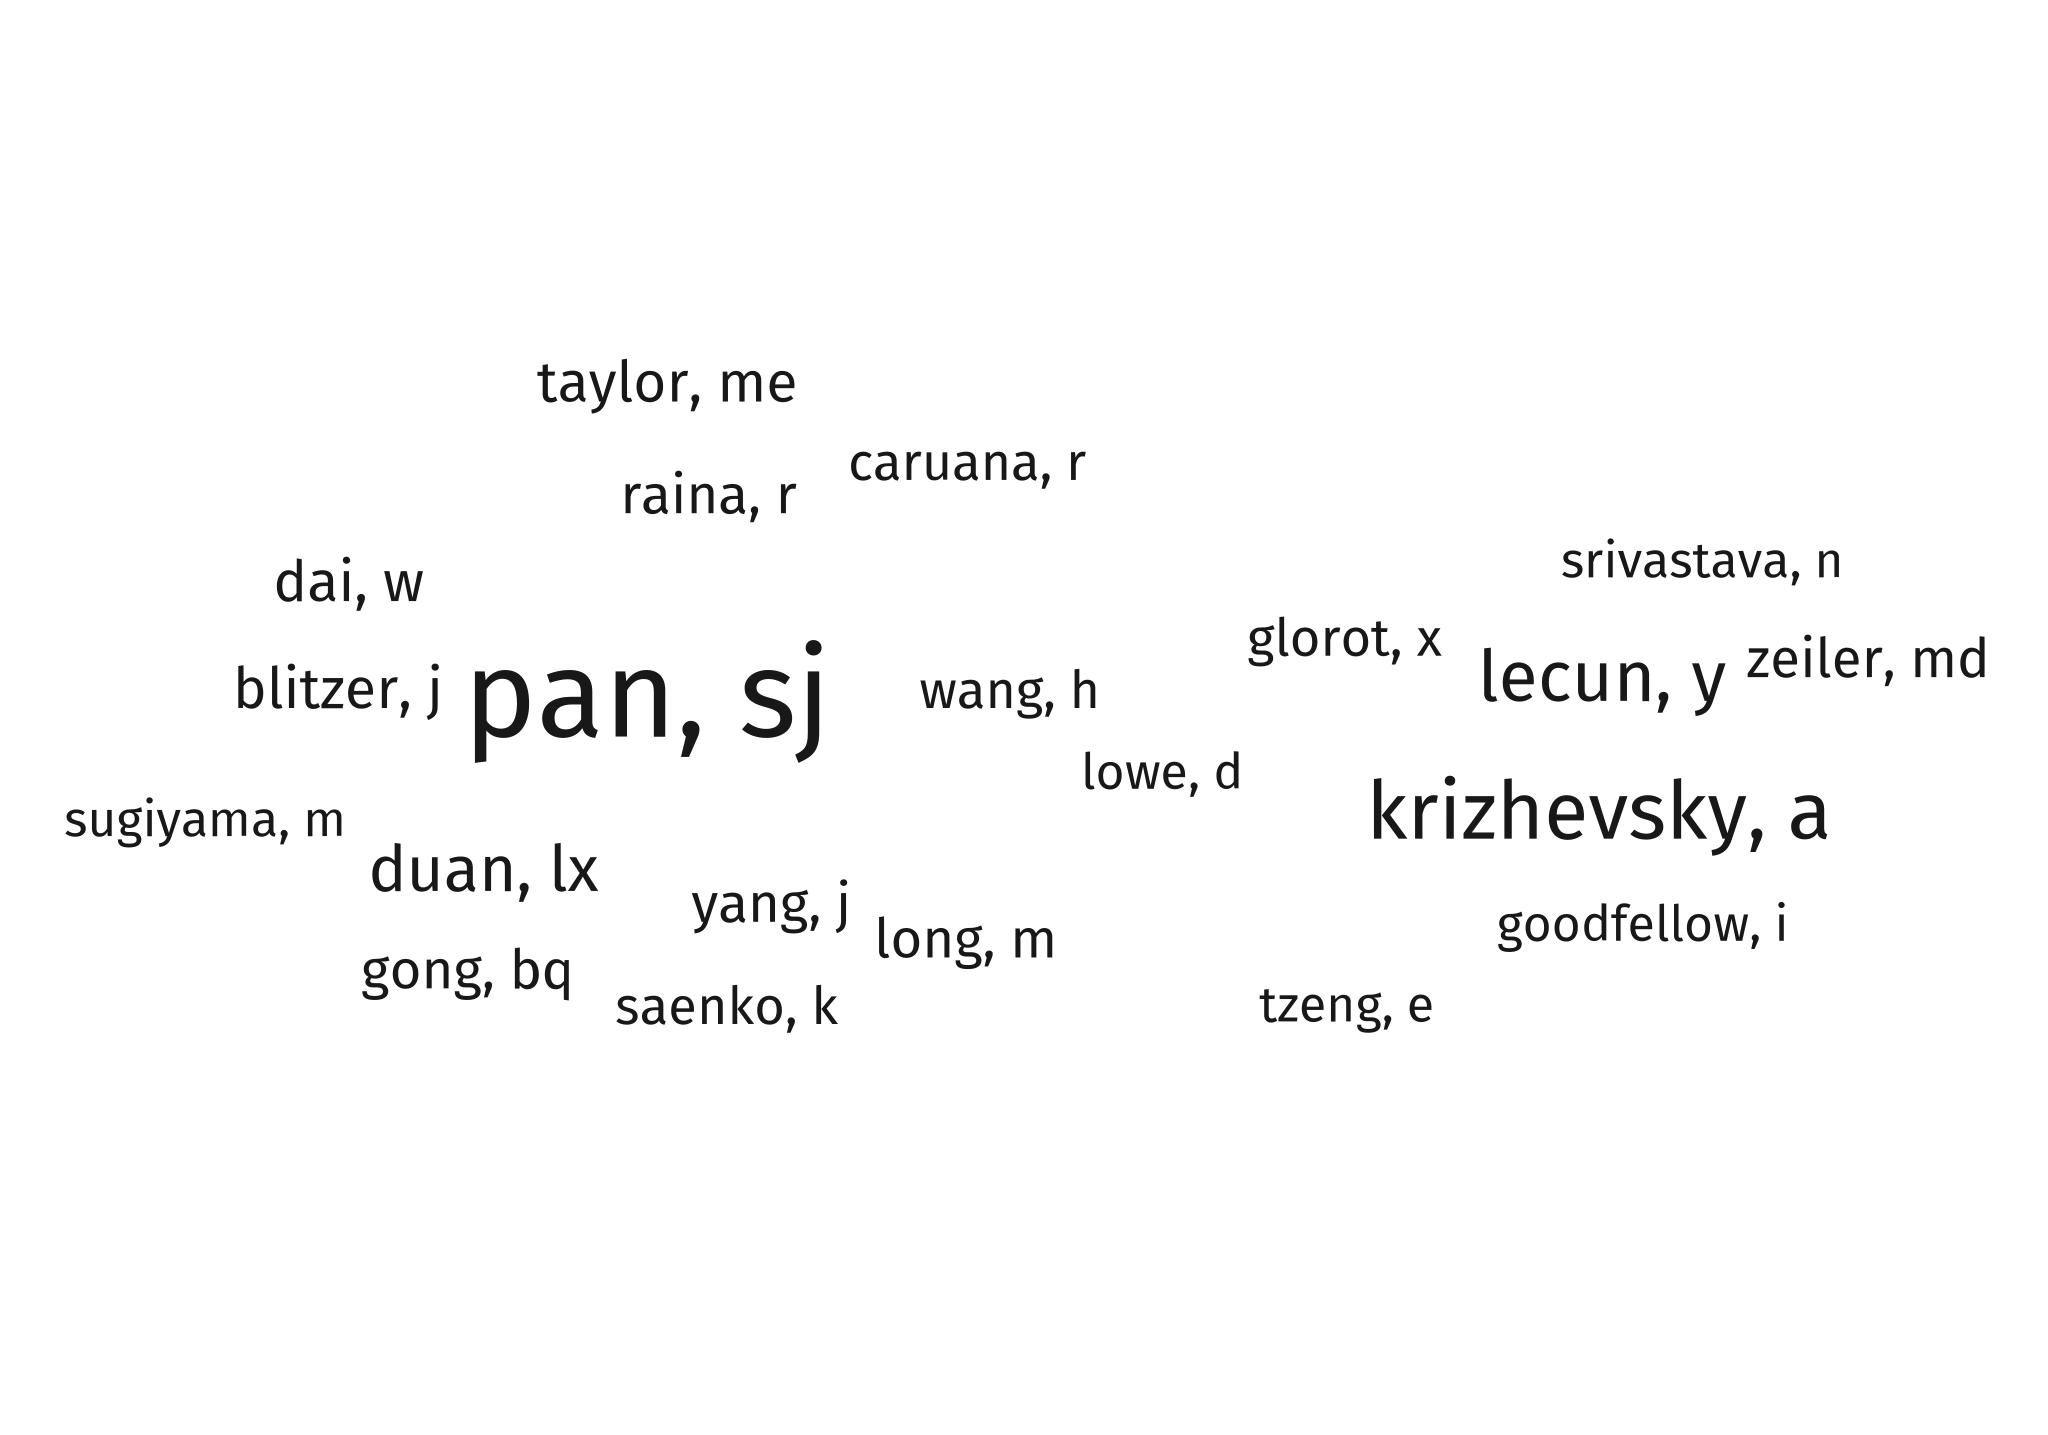
\includegraphics[width=\columnwidth]{completo-4clusters}}
    \source{Web of Science (março/2019)}{VosViewer\protect{~\cite{VOSviewer}}}
    \caption{Núcleos de conhecimento obtidos pela análise de co-citações. Os diferentes grupos representam autores que normalmente são co-citados nos 1268 artigos resultantes da busca realizada.}
    \label{fig:classicos}
  \end{figure}
  

  \lipsum[3]
  \begin{figure}
    \fbox{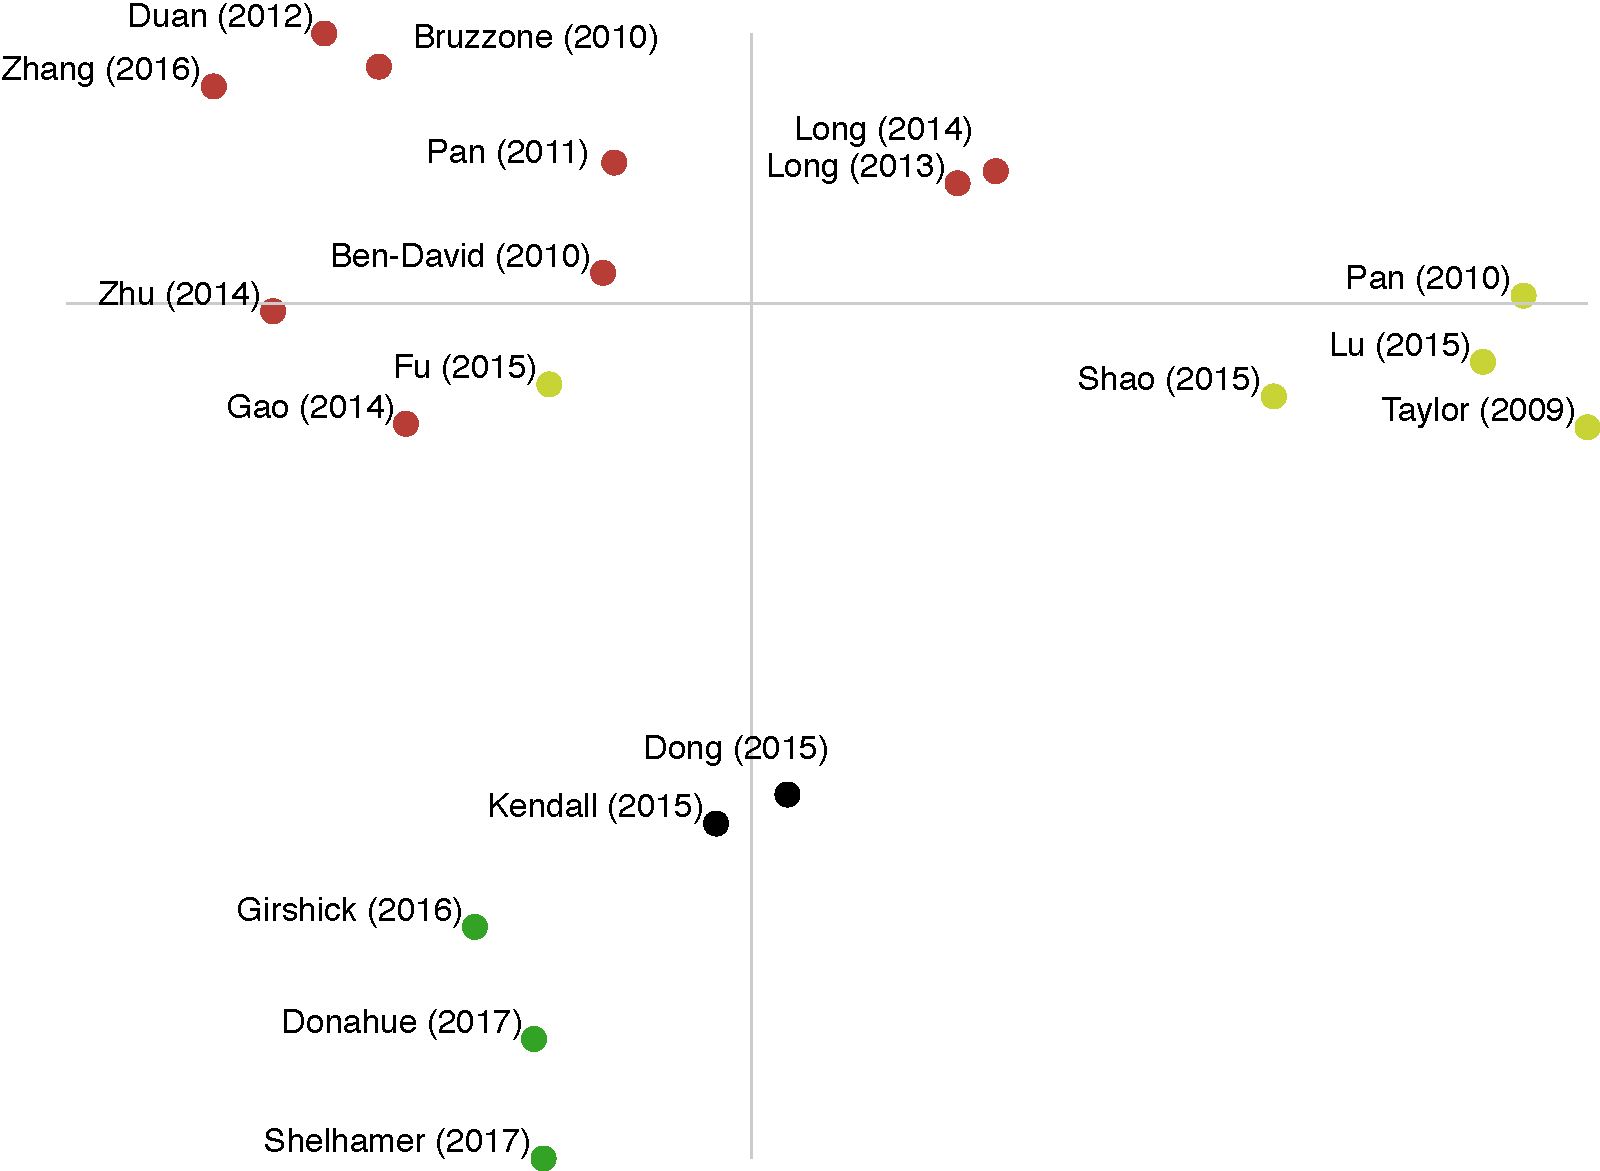
\includegraphics[width=\columnwidth]{top20_scatter.pdf}}
    \caption{} \label{fig:studysite}
  \end{figure}
  
  \subsection{A Fronteira}\label{fronteira}
  \lipsum[2]
  \begin{figure}
    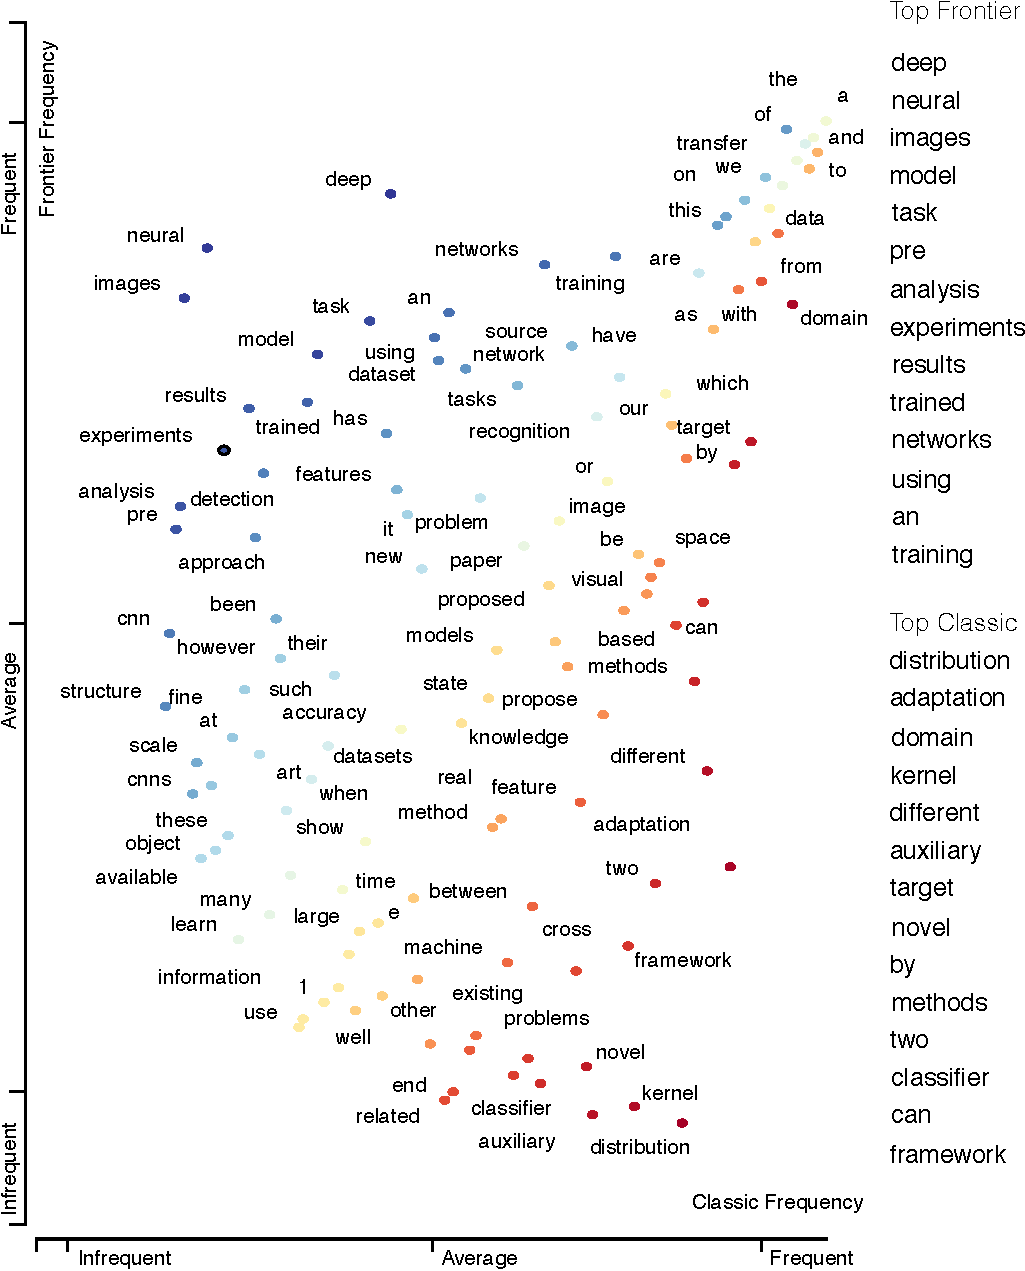
\includegraphics[width=\columnwidth]{frontier3.pdf}
    \caption{} \label{fig:scatterText}
  \end{figure}

\section{Problemas em Aberto}
\begin{enumerate}
  \item inexistência de métricas específicas para medir transferência.
  \item não há uma categorização que dê a devida importância a métodos mais novos (GANs, autoencoders)...???
  \item NLP
  \item Teoria
  \item categorização específica deep transfer learning
  \item 
\end{enumerate}
\lipsum[3]
\section{Conclusão}
\lipsum[3]
\bibliographystyle{ACM-Reference-Format}
\bibliography{references}
\end{document}
